% ============================================================
% Reporte: datapath-3
% Generado a partir de reportes/comun/plantilla_base.tex
% (NO edites la plantilla: cada unidad trabaja en su main.tex)
%
% Reglas de secciones y extensiones: reportes/AGENTS.md
% Compilar SIEMPRE con:
%   ../../scripts/latexbuild main.tex      (desde esta carpeta)
%   → genera build/main.pdf
% ============================================================
\documentclass[llncs]{llncs}

\usepackage[utf8]{inputenc}
\usepackage[T1]{fontenc}
\usepackage{fontspec}
\setmonofont{DejaVu Sans Mono}
\usepackage{graphicx}
\usepackage{listings}
\usepackage{hyperref}
\usepackage{xcolor}

% ---- Estilo para código VHDL (apéndice y fragmentos) ----
\lstdefinestyle{vhdl}{
  language=VHDL,
  basicstyle=\ttfamily\scriptsize,
  keywordstyle=\color{black},
  commentstyle=\color{gray}\itshape,
  stringstyle=\color{black},
  showstringspaces=false,
  breaklines=true,
  frame=single,
  rulecolor=\color{black}
}
\lstset{style=vhdl}

% ---- Estilo para pseudocódigo ----
\lstdefinestyle{pseudocodigo}{
  basicstyle=\ttfamily\footnotesize,
  keywordstyle=\color{black}\bfseries,
  commentstyle=\color{gray}\itshape,
  showstringspaces=false,
  breaklines=true,
  frame=single,
  rulecolor=\color{black},
  columns=fullflexible
}

\begin{document}

% ============================================================
% TÍTULO Y AUTORES
% ============================================================
\title{Diseño y Verificación de un Datapath de 8 Bits con Unidad de Control Microprogramada en {VHDL}}

\author{Aldo Mauricio Villegas Peralta$^{1}$,%
\and Uriel Lemus Pérez$^{1}$,%
\and Max Ramos Martínez$^{1}$,%
\and Alfredo Ramírez Candia$^{1}$,%
\and Santiago Silverio Flores$^{1}$}

\authorrunning{Villegas Peralta et al.}
\institute{Equipo de Arquitectura de Computadoras,\\
Benemérita Universidad Autónoma de Puebla, Puebla, México\\
\email{\{vp202368617, lp202362797, rm202376182, rc202375947, sf202367190\}@alm.buap.mx}}

\maketitle

% ============================================================
% RESUMEN  (< 100 palabras)
% ============================================================
\begin{abstract}
Resumen. Se diseña e implementa en VHDL-2008 un datapath de 8 bits sin
signo con unidad de control basada en una ROM de microinstrucciones,
siguiendo el esquema de la asignatura. El sistema se valida con 14 bancos
de prueba autochequeados en GHDL y capturas en GTKWave, cubriendo cuatro
experimentos: suma acumulada de 1..n, factorial, multiplicación $A \times
B$ y sucesión de Fibonacci. Todos los bancos pasan; se miden los
microciclos de cada caso (p.\ ej.\ $5! = 120$ en 145 microciclos,
$F(13) = 233$ en 130) y se documenta una corrección del algoritmo de
Fibonacci detectada por simulación.
\end{abstract}

\noindent\textbf{Palabras Clave:} Arquitectura de Computadoras, Datapath,
Unidad de Control, Microprogramación, VHDL, GHDL

% ============================================================
% 1. INTRODUCCIÓN
% ============================================================
\section{Introducción}
\label{sec:intro}

La organización de un procesador se concibe habitualmente como la
composición de dos subsistemas complementarios: la \emph{ruta de datos}
(datapath), que mueve y transforma los operandos a través de registros,
buses y una unidad lógico-aritmética, y la \emph{unidad de control}, que
especifica en cada instante qué microoperación se ejecuta
\cite{hamacher2002co}. Esta separación conceptual es el hilo conductor de
cualquier curso de arquitectura moderna: en las implementaciones de ciclo
único de un procesador, el datapath y el control se diseñan de forma
conjunta pero se describen por separado, de modo que el control se reduce
a una máquina de estados que genera las señales de habilitación del
datapath \cite{patterson2017cod}. Una variante clásica de ese control es
la \emph{microprogramación}: en lugar de codificar la lógica de control en
combinacional puro, cada estado de la máquina produce una palabra
(microinstrucción) almacenada en una memoria ROM, lo que simplifica el
diseño y permite inspeccionar y modificar el comportamiento sin tocar el
hardware \cite{bryant2015csapp}.

El diseño de estas estructuras se apoya en la constante reducción del
coste del silicio: el número de transistores disponibles se duplica de
forma periódica, de manera que componentes que antes exigían un esfuerzo
de integración enorme hoy se describen en pocas líneas de un lenguaje de
descripción de hardware \cite{wiki-moore}. En este trabajo se aprovecha
precisamente esa facilidad: todo el sistema se escribe en VHDL-2008
\cite{ieee1076_2008}, un estándar formal y legible tanto por máquinas como
por personas, y se verifica por simulación antes de cualquier
implementación física.

El objetivo del trabajo es diseñar, implementar y verificar
experimentalmente un datapath completo de 8 bits sin signo, con su unidad
de control microprogramada, capaz de ejecutar cuatro algoritmos clásicos
de la asignatura: la suma acumulada $S(n) = \sum_{i=1}^{n} i$, el
factorial $n!$, la multiplicación por suma repetida $A \times B$ y la
sucesión de Fibonacci $F(n)$. Cada algoritmo se ejecuta sobre el mismo
hardware, seleccionado por un código de modo, de modo que la ROM de
microinstrucciones contiene cuatro ``programas'' distintos. El coste de
cada ejecución se cuantifica en microciclos, siguiendo la idea de medir
el rendimiento de un diseño por sus ciclos \cite{stallings2015coa} y los
principios cuantitativos de coste y rendimiento de
\cite{hennessy2017qa}.

El artículo se organiza así. La Sección~\ref{sec:diseno} describe el
marco teórico y el diseño de cada módulo VHDL, incluida la ROM de
microinstrucciones. La Sección~\ref{sec:propuesta} presenta la
metodología experimental (GHDL, GTKWave y los bancos de prueba). La
Sección~\ref{sec:simulaciones} muestra las capturas de ondas de los cuatro
experimentos; la Sección~\ref{sec:resultados} analiza los resultados
cuantitativos y cualitativos, y la Sección~\ref{sec:conclusiones} cierra
con las conclusiones y el trabajo futuro. El Apéndice~\ref{app:codigo}
reproduce el código VHDL completo.

% ============================================================
% 2. DISEÑO TEÓRICO
% ============================================================
\section{Diseño Teórico}
\label{sec:diseno}

\subsection{Arquitectura general}
\label{sec:arquitectura}

El datapath implementa el esquema de la Fig.~\ref{fig:arquitectura},
proporcionado en la asignatura. En el centro se encuentra un
\emph{acumulador} de 8 bits que funciona como registro de propósito
general del sistema: casi todas las microoperaciones leen su salida
(\texttt{bus\_acc}) y, cuando corresponde, capturan un nuevo valor en el
flanco de reloj. Sobre él se apoyan dos caminos de selección:

\begin{itemize}
  \item un \textbf{multiplexor superior} de cuatro entradas que alimenta
    la entrada del acumulador: los operandos externos (\texttt{ext1},
    \texttt{ext2}), la salida del banco de registros y la realimentación
    del corrimiento;
  \item un \textbf{multiplexor inferior} de dos entradas que elige entre
    la salida de la ALU y la propia salida del acumulador para
    escribir en el banco de registros.
\end{itemize}

\noindent A la derecha del acumulador se sitúan los consumidores de
\texttt{bus\_acc}: la \textbf{ALU} (cuya entrada B proviene del banco de
registros), el \textbf{banco de registros} de $8 \times 8$ bits con un
solo puerto de lectura/escritura, y el \textbf{buffer de salida} con
habilitación tri-estado que expone el resultado al exterior. A la
izquierda, la salida de la ALU atraviesa el multiplexor inferior, un
\textbf{corrimiento} y un \textbf{detector de cero}, y se realimenta al
multiplexor superior: de este modo el resultado de cualquier operación
puede volver al acumulador en el siguiente microciclo, incluidos los
valores corregidos. El detector de cero genera el flag \texttt{cero} que
la unidad de control usa para sus saltos condicionales.

\begin{figure}[t]
  \centering
  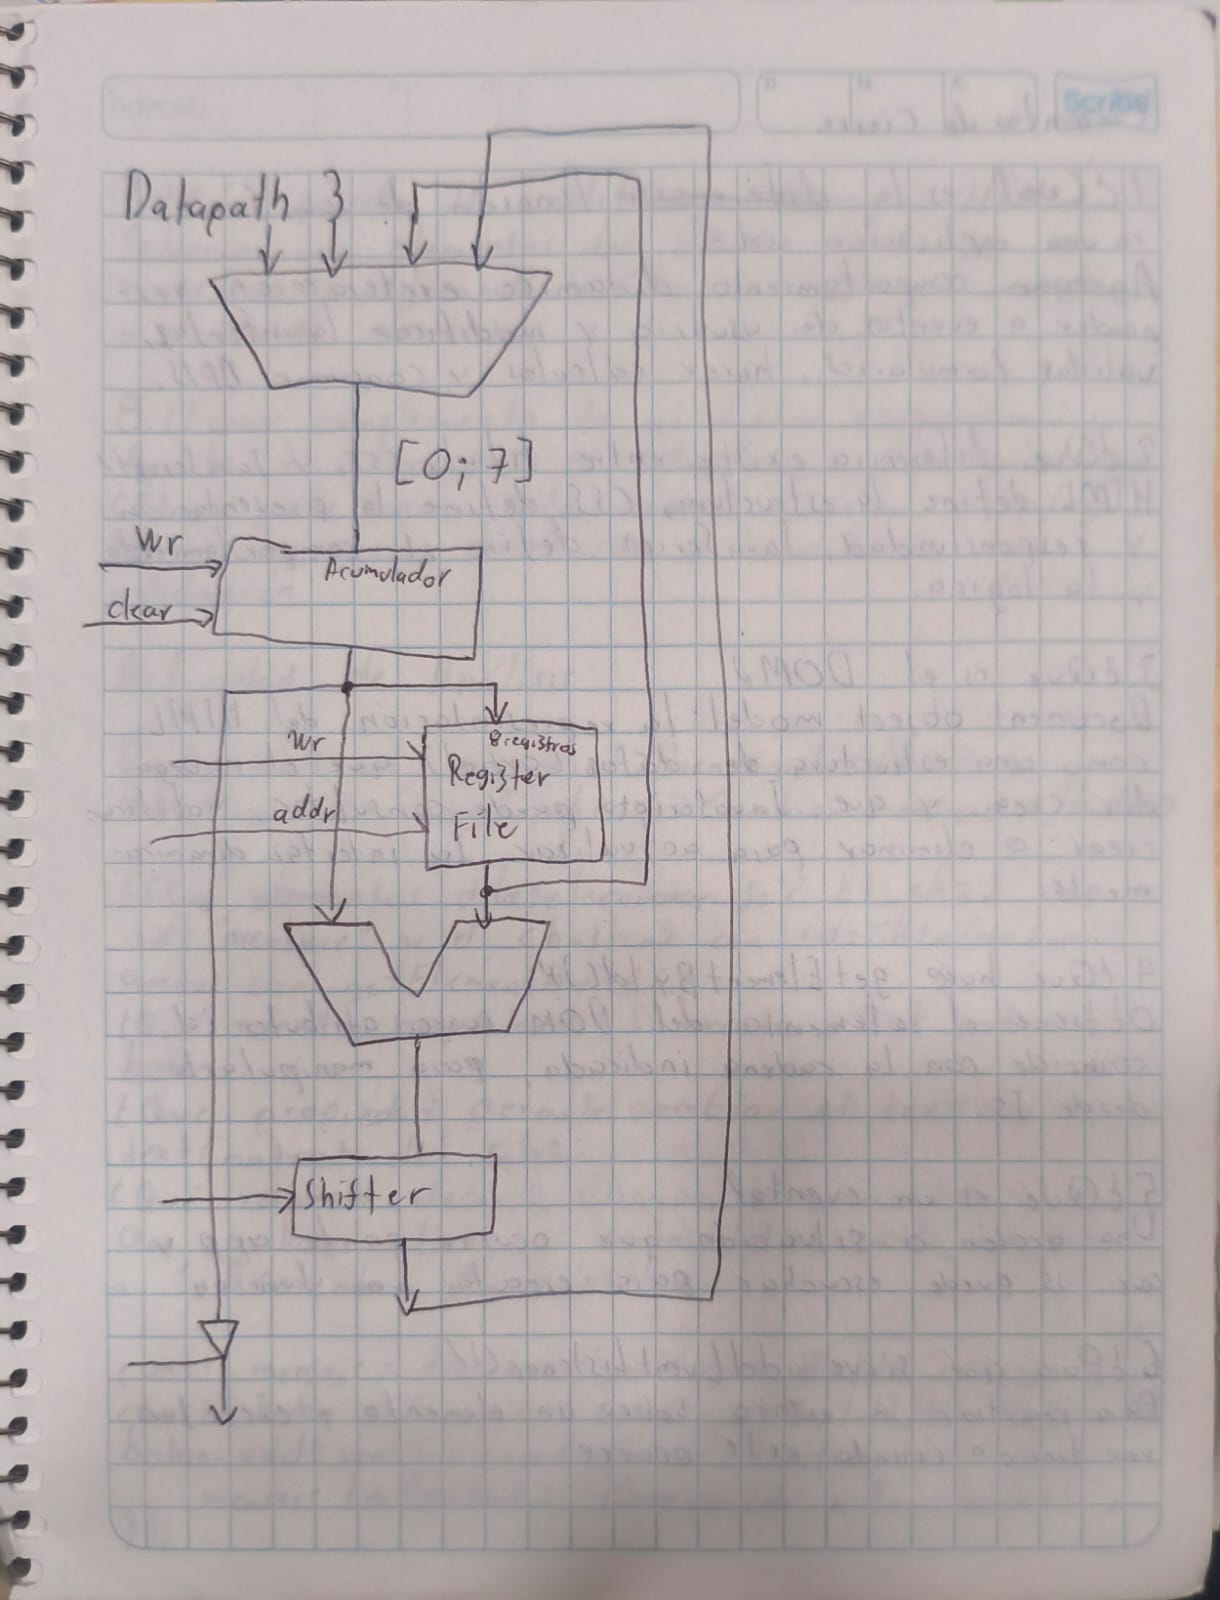
\includegraphics[width=0.85\textwidth]{figuras/arquitectura-datapath-3.jpeg}
  \caption{Esquema del datapath proporcionado en la asignatura. Se
  observan el acumulador central, el multiplexor superior de cuatro
  entradas, el banco de registros, la ALU, el multiplexor inferior, el
  corrimiento con detección de cero y el buffer de salida.}
  \label{fig:arquitectura}
\end{figure}

Todas las operaciones son \emph{sin signo} sobre 8 bits: los resultados
se reducen módulo $2^8$, sin gestión de acarreo ni de banderas de
desbordamiento \cite{patterson2017cod}. Esta decisión acota el rango
útil de cada algoritmo (Sección~\ref{sec:resultados}) pero simplifica el
diseño y deja el enfoque en el control, que es el objetivo didáctico del
trabajo.

\subsection{Módulos de la ruta de datos}
\label{sec:modulos}

El diseño se descompone en diez entidades VHDL, una por fichero, todas
con la lógica resoluble \texttt{std\_logic} del paquete IEEE 1164
\cite{ieee1164_1993} y aritmética sin signo de \texttt{numeric\_std}
\cite{ashenden2008vhdl}. Los estilos de descripción se combinan según
conviene: \emph{dataflow} para los multiplexores y la ALU,
\emph{behavioral} para el acumulador, el banco y la control, y
\emph{estructural} para el datapath integrado, siguiendo las
recomendaciones de modelado de \cite{navabi1998vhdl} y
\cite{brown2009fdld}.

\paragraph{ALU.}
La ALU de 8 bits (\texttt{alu.vhd}) recibe el operando A del acumulador
y el operando B del banco de registros, y decodifica ocho operaciones
con un campo de tres bits (Tabla~\ref{tab:alu}). Los bloques
aritméticos (suma, resta, incremento y decremento) y el corrimiento
responden a los principios de diseño de datapaths aritméticos descritos
en \cite{rabaey2002dic}; la resta se obtiene como suma del complemento
a dos, con reducción módulo 256.

\begin{table}[t]
\centering
\caption{Código de operación de la ALU (campo \texttt{op\_alu}).}
\label{tab:alu}
\begin{tabular}{cll}
\hline
\texttt{op} & Operación & Descripción \\
\hline
000 & Pasar A     & $f = A$ (no nula) \\
001 & $A + B$     & suma \\
010 & $A - B$     & resta \\
011 & $A + 1$     & incremento \\
100 & $A - 1$     & decremento \\
101 & $A \lor B$  & OR bit a bit \\
110 & $A \land B$ & AND bit a bit \\
111 & $\lnot A$   & NOT de A \\
\hline
\end{tabular}
\end{table}

\paragraph{Acumulador.}
El acumulador (\texttt{acumulador.vhd}) es un registro de 8 bits con dos
entradas de control: \texttt{wr\_acc} escribe el valor del multiplexor
superior y \texttt{clear\_acc} reinicia a cero. Cuando ambas se activan
a la vez, el \emph{clear} tiene prioridad, convención habitual de los
registros con reinicio asíncrono dominante \cite{harris2015ddca}.

\paragraph{Banco de registros.}
El banco (\texttt{banco\_registro.vhd}) almacena ocho registros de 8
bits con un único puerto: la dirección \texttt{addr} selecciona qué
registro se escribe (cuando \texttt{wr\_rf} está activo) o qué registro
se lee en \texttt{rf\_dout} (en modo lectura). Esta organización de un
solo puerto obliga a la microprogramación a separar en el tiempo la
escritura y la lectura de un mismo registro, restricción que se refleja
directamente en las tablas de microinstrucciones.

\paragraph{Multiplexores, corrimiento, detector de cero y buffer.}
El multiplexor superior (\texttt{mux\_superior.vhd}) codifica cuatro
fuentes con \texttt{sel\_sup}: dos externas, el banco y la
realimentación; la entrada \texttt{ext2} se deja cableada a cero por
simplicidad. El multiplexor inferior (\texttt{mux\_inferior.vhd}) elige
entre ALU y acumulador para las escrituras en el banco. El corrimiento
(\texttt{shifter.vhd}) soporta paso idéntico (\texttt{sh} = 00, el modo
usado por los cuatro experimentos), corrimiento lógico a la izquierda y
a la derecha; la señal de salida es también la que alimenta al detector
de cero (\texttt{detector\_cero.vhd}), de modo que el flag indica
\emph{si el valor que entra en el acumulador en el siguiente flanco será
cero}, decisión tomada en la Sección~\ref{sec:control}. Por último, el
buffer de salida (\texttt{buffer\_salida.vhd}) es una compuerta
tri-estado: solo cuando \texttt{out\_en} está activo, \texttt{dato\_out}
refleja el acumulador; en caso contrario queda en alta impedancia,
permitiendo compartir el bus de resultados \cite{wakerly2005ddpp},
\cite{wiki-tristate}.

\paragraph{Corrimiento barrel.}
Aunque los experimentos usan el paso idéntico, el shifter está
concebido como un corrimiento por N posiciones en un solo ciclo, es
decir, un \emph{barrel shifter} \cite{wiki-barrel}, patrón habitual en
los datapaths aritméticos \cite{rabaey2002dic}.

\paragraph{Datapath integrado.}
La entidad \texttt{datapath.vhd} instancia los ocho bloques anteriores
por componentes, conecta el \texttt{ext\_data} de entrada al
multiplexor superior y expone, además de los buses, las señales de
control y el flag \texttt{cero}. La instanciación por componentes (en
lugar de por entidad directa) mantiene el orden de análisis
independiente del orden de los ficheros, práctica recomendada para
flujos de compilación por lotes \cite{ashenden2008vhdl}.

\subsection{Unidad de control}
\label{sec:control}

La unidad de control (\texttt{control.vhd}) es una máquina de estados
\cite{wiki-fsm} de un microciclo por flanco: en cada flanco de reloj
avanza al siguiente paso y aplica la palabra que la ROM devuelve para
ese paso. El estado se codifica en dos campos: \texttt{modo} (dos bits,
selecciona el experimento) y \texttt{paso} (siete bits). La dirección de
la ROM se forma como $\texttt{modo} \times 32 + \texttt{paso}$, de modo
que cada experimento dispone de hasta 32 microinstrucciones
contiguas, con base $0$, $32$, $64$ y $96$ para los modos 00, 01, 10 y
11 respectivamente.

Cada microinstrucción contiene los campos de la
Tabla~\ref{tab:microinstruccion}. Las operaciones de escritura en el
acumulador, el banco y el buffer son mutuamente excluivas por
construcción del codificador; el campo \texttt{dir} codifica tanto la
dirección de salto incondicional (\texttt{salta}) como la del salto
condicional (\texttt{salto\_si\_cero}), y \texttt{fin} detiene el
contador de pasos y marca el final de la ejecución. La señal
\texttt{ciclos} de 16 bits expone el número de microciclos transcurridos,
lo que permite medir el coste de cada experimento sin instrumentación
externa \cite{stallings2015coa}.

\begin{table}[t]
\centering
\caption{Campos de una microinstrucción de la ROM de control.}
\label{tab:microinstruccion}
\begin{tabular}{cll}
\hline
Campo & Anchura & Función \\
\hline
\texttt{sel\_sup}  & 2 & fuente hacia el acumulador \\
\texttt{wr\_acc}   & 1 & escribe el acumulador \\
\texttt{clr\_acc}  & 1 & limpia el acumulador \\
\texttt{addr}      & 3 & dirección del banco de registros \\
\texttt{wr\_rf}    & 1 & escribe el banco de registros \\
\texttt{op\_alu}   & 3 & operación de la ALU (Tabla~\ref{tab:alu}) \\
\texttt{sel\_inf}  & 1 & 0: ALU, 1: acumulador hacia el banco \\
\texttt{sh}        & 2 & modo del corrimiento \\
\texttt{out\_en}   & 1 & habilita el buffer de salida \\
\texttt{salta}     & 1 & salto incondicional a \texttt{dir} \\
\texttt{salto\_si\_cero} & 1 & salta a \texttt{dir} si el flag está activo \\
\texttt{fin}       & 1 & termina la ejecución \\
\texttt{dir}       & 7 & dirección destino \\
\hline
\end{tabular}
\end{table}

El salto condicional muestrea el flag \texttt{cero} \emph{durante} el
microciclo en que la ALU calcula el resultado, es decir, en el mismo
flanco en que el acumulador lo captura. Esta sincronía es una decisión
delicada y consciente: como el detector es combinacional, su valor deja
de ser representativo justo después del flanco, cuando el acumulador ya
contiene el nuevo dato. Modelar correctamente esta relación entre
combinacional y secuencial es un punto central del diseño de FSM
sincrónicas \cite{mano2016lcdf}, \cite{harris2015ddca},
\cite{roth2013fld}; una lectura tardía del flag produciría saltos
falsos. El resto de la lógica de control (decodificación, contador de
pasos y banderas de fin) se describe con procesos y sentencias
secuenciales al estilo de \cite{ashenden2008vhdl} y las FSM registradas
de \cite{katz2005cld}.

\subsection{Algoritmos de los experimentos}
\label{sec:algoritmos}

Los cuatro algoritmos comparten el mismo hardware y se seleccionan con
\texttt{modo}. El pseudocódigo siguiente corresponde a la secuencia de
microinstrucciones efectivamente grabada en la ROM (el desglose completo
de filas está en el código del Apéndice~\ref{app:codigo}).

\paragraph{Exp.\ 1 --- Suma de $1 \dots n$ (modo 00).}
$S$ se acumula en el banco y $i$ cuenta descendentemente:
\begin{lstlisting}[style=pseudocodigo]
S <- 0 ; i <- n
si i = 0 -> fin
bucle: S <- S + i ; i <- i - 1
        si i = 0 -> fin          # paso la salida al buffer
        ir a bucle
\end{lstlisting}

\paragraph{Exp.\ 2 --- Factorial (modo 01).}
Se mantiene el producto parcial en el banco; $k$ decrece desde $n$:
\begin{lstlisting}[style=pseudocodigo]
p <- 1 ; k <- n
si k = 0 -> fin                  # 0! = 1
bucle: p <- p * k ; k <- k - 1   # la multiplicacion es un
        si k = 0 -> fin          #   sub-bucle interno
        ir a bucle
\end{lstlisting}

\paragraph{Exp.\ 3 --- Multiplicación $A \times B$ (modo 10).}
Suma repetida: se suman $B$ unidades, $A$ veces:
\begin{lstlisting}[style=pseudocodigo]
p <- 0 ; i <- A
si i = 0 -> fin                  # 0 x B = 0
bucle: p <- p + B ; i <- i - 1
        si i = 0 -> fin
        ir a bucle
\end{lstlisting}

\paragraph{Exp.\ 4 --- Fibonacci (modo 11).}
Dos registros mantienen el par $(a, b) = (F(k), F(k+1))$; con la
inicialización $a=0$, $b=1$, cada iteración deja $b = F(k+1)$, por lo
que el bucle debe ejecutarse $n-1$ veces para $n \ge 1$ (los casos
$n=0$ y $n=1$ salen antes del bucle). Esta corrección fue detectada
por simulación (Sección~\ref{sec:resultados}).
\begin{lstlisting}[style=pseudocodigo]
a <- 0 ; b <- 1
si n = 0 -> fin_a                # F(0) = a
si n = 1 -> fin_b                # F(1) = b
veces <- n - 1
bucle: next <- a + b ; a <- b ; b <- next
        veces <- veces - 1 ; si cero -> fin_b
        ir a bucle
fin_a: Acc <- a
fin_b: Acc <- b
\end{lstlisting}

% ============================================================
% 3. PROPUESTA EXPERIMENTAL
% ============================================================
\section{Propuesta Experimental}
\label{sec:propuesta}

La verificación se realizó por simulación con dos herramientas libres:
GHDL, un simulador VHDL-2008 con analizador, elaborador y ejecutor
\cite{ghdl-docs}, y GTKWave, un visor de ondas que lee los volcados
VCD generados por GHDL \cite{gtkwave-docs}. Ambas se invocan
exclusivamente a través de los scripts del repositorio
(\texttt{scripts/vhdl-analizar}, \texttt{scripts/vhdl-sim} y
\texttt{scripts/vhdl-wave}), que fijan el estándar \texttt{--std=08} y
la ruta de salidas.

La estrategia de bancos de prueba \emph{autochequeados} se aplicó en
cuatro niveles, de abajo hacia arriba:

\begin{enumerate}
  \item \textbf{Módulos (8 bancos).} Cada uno de los ocho bloques
    básicos tiene su banco (\texttt{tb\_alu}, \texttt{tb\_acumulador},
    \texttt{tb\_banco\_registros}, \texttt{tb\_mux\_superior},
    \texttt{tb\_mux\_inferior}, \texttt{tb\_shifter},
    \texttt{tb\_detector\_cero}, \texttt{tb\_buffer\_salida}) con
    \texttt{assert ... severity failure} en cada valor esperado.
  \item \textbf{Integración (1 banco).} \texttt{tb\_datapath} aplica
    microoperaciones una a una sobre el datapath completo, comprobando
    cada bus y el flag de cero.
  \item \textbf{Control (1 banco).} \texttt{tb\_control} verifica que la
    ROM reproduce exactamente las secuencias de los cuatro experimentos
    (con el flag forzado para ejercitar ambos caminos del salto) y que
    ningún experimento termina en 100 microciclos si el flag nunca se
    activa.
  \item \textbf{Experimentos (4 bancos).} \texttt{tb\_exp1\_suma},
    \texttt{tb\_exp2\_factorial}, \texttt{tb\_exp3\_mult} y
    \texttt{tb\_exp4\_fibonacci} integran datapath y control con cada
    modo, cargan los operandos por el puerto externo, esperan la señal
    \texttt{fin}, leen el resultado por \texttt{dato\_out} y comparan
    contra el valor esperado. Además imprimen el número de microciclos
    (\texttt{report}) para el análisis de la Sección~\ref{sec:resultados}.
\end{enumerate}

\noindent La matriz de pruebas se eligió para cubrir los casos límite y
algunos valores intermedios: $n \in \{1, 3, 5\}$ en la suma;
$n \in \{1, 5\}$ en el factorial; $(A, B) \in \{(4,3), (5,5),
(15,15)\}$ en la multiplicación; y $n \in \{0, 1, 7, 13\}$ en Fibonacci,
incluyendo $F(0)$ (camino de salida sin bucle) y $F(13) = 233$, el mayor
valor que cabe en 8 bits. El código de referencia de cada banco es el
Apéndice~\ref{app:codigo}.

Para la sección de capturas, cada volcado VCD se cargó en GTKWave con un
script Tcl que selecciona las señales de interés, aplica modo blanco y
negro (contraste óptimo para impresión en escala de grises) y ajusta la
vista al intervalo completo; el PNG resultante se recortó a los
límites del panel de ondas con una utilidad propia incluida en el
repositorio.

% ============================================================
% 4. SIMULACIONES DE VHDL
% ============================================================
\section{Simulaciones de VHDL}
\label{sec:simulaciones}

Las Figs.~\ref{fig:exp1}--\ref{fig:exp4} muestran las ondas de los
cuatro experimentos. En todas ellas se observan, de arriba hacia abajo:
el modo seleccionado, el paso de la ROM, el acumulador, la salida del
banco de registros, la salida del buffer (en alta impedancia hasta que
\texttt{fin} activa \texttt{out\_en}), las señales de selección de los
multiplexores, el código de la ALU, la dirección del banco, la escritura
del banco y el par \texttt{cero}/\texttt{fin}. Las tres ``ventanas''
de actividad separadas corresponden a los tres (o cuatro) casos de
prueba de cada experimento.

\begin{figure}[t]
  \centering
  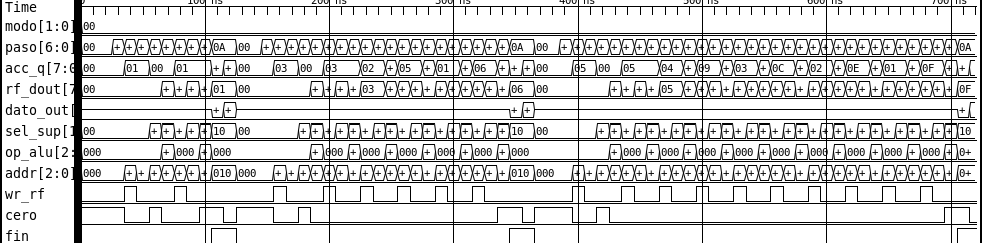
\includegraphics[width=\textwidth]{figuras/exp1-suma-ondas.png}
  \caption{Experimento 1 --- Suma de $1 \dots n$ (modo 00). Casos
  $n=1$, $n=3$ y $n=5$. Se observa el bucle de seis microciclos por
  iteración y la salida del resultado en \texttt{dato\_out} al final de
  cada caso.}
  \label{fig:exp1}
\end{figure}

\begin{figure}[t]
  \centering
  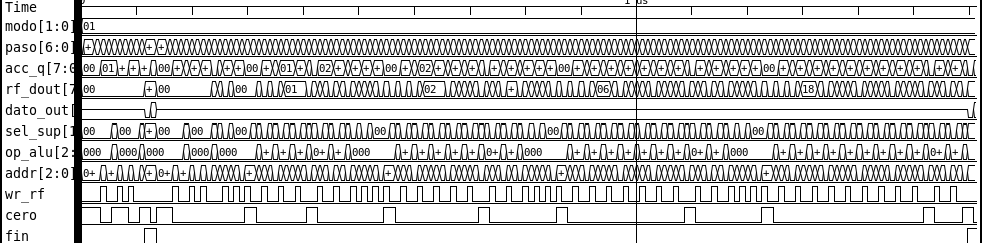
\includegraphics[width=\textwidth]{figuras/exp2-factorial-ondas.png}
  \caption{Experimento 2 --- Factorial (modo 01). Casos $n=1$ y $n=5$.
  La actividad densa corresponde al sub-bucle de multiplicación por
  suma repetida embebido en cada iteración del factorial.}
  \label{fig:exp2}
\end{figure}

\begin{figure}[t]
  \centering
  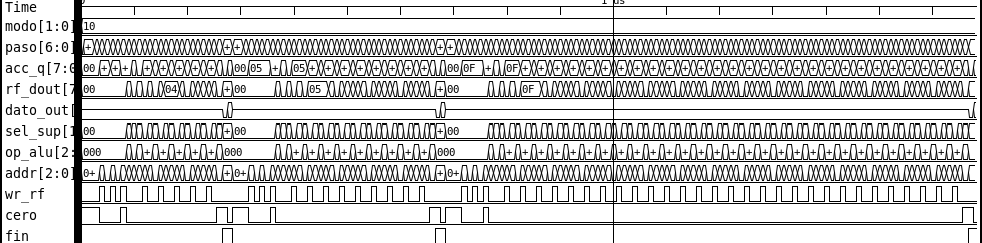
\includegraphics[width=\textwidth]{figuras/exp3-multiplicacion-ondas.png}
  \caption{Experimento 3 --- Multiplicación $A \times B$ (modo 10).
  Casos $(4,3)$, $(5,5)$ y $(15,15)$. El bucle exterior recorre $A$
  iteraciones de suma de $B$.}
  \label{fig:exp3}
\end{figure}

\begin{figure}[t]
  \centering
  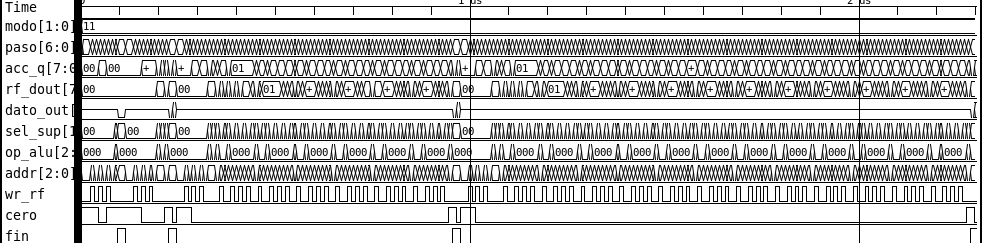
\includegraphics[width=\textwidth]{figuras/exp4-fibonacci-ondas.png}
  \caption{Experimento 4 --- Fibonacci (modo 11). Casos $n=0$, $n=1$,
  $n=7$ y $n=13$. Los dos primeros terminan antes de entrar al bucle;
  los restantes ejecutan $n-1$ iteraciones.}
  \label{fig:exp4}
\end{figure}

% ============================================================
% 5. RESULTADOS
% ============================================================
\section{Resultados}
\label{sec:resultados}

\subsection{Verificación funcional}

Los 14 bancos de prueba terminan sin violaciones de \texttt{assert},
de modo que se cumplen todos los objetivos funcionales:
Tabla~\ref{tab:resultados} resume los casos, los resultados obtenidos y
los microciclos medidos. Los cuatro algoritmos producen los valores
esperados, incluidos los extremos $0! = 1$, $F(0) = 0$, $F(1) = 1$ y
$15 \times 15 = 225$.

\begin{table}[t]
\centering
\caption{Matriz de resultados: valor esperado, valor simulado y
microciclos (puerto \texttt{ciclos}) de cada caso de prueba.}
\label{tab:resultados}
\begin{tabular}{llll}
\hline
Experimento & Caso & Resultado & Microciclos \\
\hline
Suma $1 \dots n$ & $n=1$  & $S = 1$   & 9  \\
                 & $n=3$  & $S = 6$   & 21 \\
                 & $n=5$  & $S = 15$  & 33 \\
Factorial        & $n=1$  & $1! = 1$  & 10 \\
                 & $n=5$  & $5! = 120$ & 145 \\
Multiplicación   & $4 \times 3$  & 12  & 25 \\
                 & $5 \times 5$  & 25  & 37 \\
                 & $15 \times 15$ & 225 & 97 \\
Fibonacci        & $n=0$  & $F(0) = 0$   & 8  \\
                 & $n=1$  & $F(1) = 1$   & 10 \\
                 & $n=7$  & $F(7) = 13$  & 70 \\
                 & $n=13$ & $F(13) = 233$ & 130 \\
\hline
\end{tabular}
\end{table}

\subsection{Análisis del coste}

Los microciclos permiten derivar el coste de cada algoritmo en función
de su entrada, según las métricas de rendimiento por ciclos de
\cite{stallings2015coa} y los principios cuantitativos de
\cite{hennessy2017qa}:

\begin{itemize}
  \item \textbf{Suma:} los datos $(n, \mathrm{ciclos}) = (1,9), (3,21),
    (5,33)$ ajustan exactamente a $6n + 3$: tres microciclos de
    inicialización y seis por iteración del bucle, coherente con la
    secuencia de la ROM.
  \item \textbf{Fibonacci:} para $n \ge 1$, los datos $(1,10), (7,70),
    (13,130)$ ajustan a $10n$: diez microciclos por iteración más la
    salida; $n=0$ escapa al bucle en ocho microciclos.
  \item \textbf{Factorial y multiplicación:} el coste crece con la
    entrada pero no de forma estrictamente lineal, porque la
    multiplicación embebida es a su vez un sub-bucle cuyo número de
    iteraciones depende del valor de los operandos, no solo de su
    cantidad. Así, pasar de $4 \times 3$ a $15 \times 15$ multiplica el
    coste por casi cuatro, y $5!$ exige 145 microciclos frente a los 10
    de $1!$.
\end{itemize}

\subsection{Discusión crítica}

El trabajo puso de manifiesto dos cuestiones que la sola lectura del
esquema no revela.

\paragraph{El flag de cero es combinacional.}
El detector observa la salida del corrimiento, que a su vez sale de la
ALU: su valor solo es válido \emph{durante} el microciclo, justo hasta
el flanco en que el acumulador captura el resultado. Un banco de prueba
que consultara el flag después del flanco observaría ya el valor
recalculado con el acumulador nuevo, y en concreto $0 - 1 = 255$ en el
último decremento del Exp.\ 1, lo que invalidaría la comprobación. Este
tipo de trampas de temporización entre lógica combinacional y
secuencial es justamente el contenido de los capítulos de FSM
sincrónicas de \cite{mano2016lcdf} y \cite{harris2015ddca}; el banco de
integración se ajustó para muestrear el flag al final del ciclo, como
hace la propia control.

\paragraph{Corrección del algoritmo de Fibonacci.}
La primera versión de la ROM del Exp.\ 4 ejecutaba $n$ iteraciones. La
simulación de $n=7$ devolvió $21$, que resulta ser $F(8)$, y no
$F(7) = 13$: la sucesión estaba desfasada en un término: con la
inicialización $a=0$, $b=1$, $k$ iteraciones dejan $b = F(k+1)$, no
$F(k)$. La corrección consistió en ejecutar $n-1$ iteraciones para
$n \ge 1$, dejando $n=0$ y $n=1$ como caminos de salida directa, y en
ajustar la tabla del plan de trabajo. Con la corrección, la simulación
confirma $F(7) = 13$ y $F(13) = 233$. Es un ejemplo tangible de cómo la
verificación por simulación detecta errores de especificación que la
revisión del pseudocódigo no alcanzó a ver, motivo por el cual los
bancos autochequeados forman parte del flujo oficial del repositorio.

\subsection{Límites y validez}

Al trabajar sin signo y módulo 256, cada algoritmo tiene un rango de
validez: la suma admite $n \le 22$ ($S(22) = 253$); el factorial,
$n \le 5$ ($6! = 720 > 255$); la multiplicación, $A, B \le 15$
($16 \times 16 = 256$); y Fibonacci, $n \le 13$, pues
$F(14) = 377 > 255$. Dentro de esos rangos, los 12 casos probados
cubren los extremos y confirman el comportamiento esperado; fuera de
ellos, el diseño no declara desbordamiento y el resultado se reduce
módulo 256, como se decidió en la Sección~\ref{sec:arquitectura}.

% ============================================================
% 6. CONCLUSIONES
% ============================================================
\section{Conclusiones}
\label{sec:conclusiones}

Se diseñó e implementó en VHDL-2008 un datapath completo de 8 bits con
unidad de control microprogramada, fiel al esquema de la asignatura, y
se verificó con 14 bancos de prueba autochequeados en GHDL. Los cuatro
experimentos requeridos ---suma acumulada, factorial, multiplicación y
Fibonacci--- producen los valores correctos dentro de sus rangos de
validez, y su coste en microciclos se midió y ajustó a modelos
cerrados en los casos lineales ($6n+3$ para la suma y $10n$ para
Fibonacci).

La verificación experimental demostró su valor: el desfase de un término
en el algoritmo de Fibonacci, invisible en la revisión del pseudocódigo,
se detectó y corrigió con la simulación de $n=7$; asimismo, el estudio
del flag de cero obligó a precisar el instante de muestreo del salto
condicional. Ambos hallazgos documentan el comportamiento real del
diseño y quedan cubiertos por los bancos de prueba.

Como trabajo futuro se plantea: (i) ampliar la ROM para soportar
operaciones con signo y detección de desbordamiento; (ii) sustituir el
banco de un solo puerto por uno de dos puertos y medir la reducción de
microciclos; (iii) explotar los modos de corrimiento del shifter para
implementar multiplicación desplazando y sumando, en lugar de suma
repetida; y (iv) estudiar la síntesis del diseño en una FPGA. Sobre este
último punto conviene recordar que el GHDL disponible en el entorno del
curso es una implementación \emph{mcode}, orientada a simulación, por lo
que la síntesis exigiría una herramienta adicional.

% ============================================================
% REFERENCIAS
% ============================================================
\bibliographystyle{splncs04}
\bibliography{referencias}

% ============================================================
% APÉNDICE — CÓDIGO VHDL
% ============================================================
\appendix
\section{Código VHDL}
\label{app:codigo}

Código completo de la unidad, tomado directamente de
\texttt{vhdl/datapath-3/src/} mediante \texttt{lstinputlisting}, de modo
que el apéndice permanece sincronizado con el repositorio.

\lstinputlisting[caption={alu.vhd --- unidad lógico-aritmética de 8 bits (Tabla~\ref{tab:alu})}, label=lst:alu]{../../vhdl/datapath-3/src/alu.vhd}

\lstinputlisting[caption={acumulador.vhd --- registro acumulador con escritura y clear}, label=lst:acumulador]{../../vhdl/datapath-3/src/acumulador.vhd}

\lstinputlisting[caption={banco\_registros.vhd --- banco de 8 registros de 8 bits con un solo puerto}, label=lst:banco]{../../vhdl/datapath-3/src/banco_registros.vhd}

\lstinputlisting[caption={mux\_superior.vhd --- multiplexor de cuatro fuentes hacia el acumulador}, label=lst:muxsup]{../../vhdl/datapath-3/src/mux_superior.vhd}

\lstinputlisting[caption={mux\_inferior.vhd --- multiplexor entre ALU y acumulador}, label=lst:muxinf]{../../vhdl/datapath-3/src/mux_inferior.vhd}

\lstinputlisting[caption={shifter.vhd --- corrimiento con paso idéntico (usado por los experimentos)}, label=lst:shifter]{../../vhdl/datapath-3/src/shifter.vhd}

\lstinputlisting[caption={detector\_cero.vhd --- flag de cero sobre la salida del corrimiento}, label=lst:detector]{../../vhdl/datapath-3/src/detector_cero.vhd}

\lstinputlisting[caption={buffer\_salida.vhd --- buffer tri-estado de resultados}, label=lst:buffer]{../../vhdl/datapath-3/src/buffer_salida.vhd}

\lstinputlisting[caption={datapath.vhd --- integración estructural de los ocho módulos}, label=lst:datapath]{../../vhdl/datapath-3/src/datapath.vhd}

\lstinputlisting[caption={control.vhd --- unidad de control con ROM de microinstrucciones de los cuatro experimentos}, label=lst:control]{../../vhdl/datapath-3/src/control.vhd}

\end{document}
